\chapter{Challanges of Microservices Architecture}\label{chapter:challanges_of_microservices_architecture}
\section{Introduction}\label{section:challanges_of_microservices_architecture/introduction}
The section \ref{subsection:context/monolith-disadvantages} lists some drawbacks of monolithic architecture and these have become the motivation for adopting microservices architecture. Microservices offer opportunities in various aspects however it can also be tricky to utilize them properly. It do come with few challanges. The response from interview \ref{question:hybris_architecture/interview/question_1.5} also highlights some prominent challanges. In this chapter, the challanges of microservices alongside its advantages will be discussed. \cite{Fowler:2015aa}

  \begin{multicols}{2}
  \textbf{\underline{Advantages}} 
  \vfill
  \columnbreak
  \textbf{\underline{Challanges}}
  \end{multicols}
  \begin{multicols}{2}
  \textbf{Strong Modular Boundaries} \\It is not totally true that monolith have weaker modular structure than microservices but it is also not false to say that as the system gets bigger, it is very easy for monolith to turn in to a big ball of mud. However, it is very difficult to do the same with microservices. Each microservice is a cohesive unit with full control upon its business entities. The only way to access its data is through its \acrshort{API}.
  \vfill
  \columnbreak
  \textbf{Distributed System} \\The infrastructure of microservices is distributed, which brings many complications alongside, as listed by 8 fallacies.\cite{Factor:2014aa} The calls are remote which are imminent to accomplish business goals. The remote calls are slower than local and affect performance in a great deal. Additionally, network is not reliable which makes it challanging to accept and handle the failures.
  \end{multicols}

\begin{multicols}{2}
  \textbf{Independent Deployment} \\Due the nature of microservices being autonomous components, each microservice can be deployed independently. Deployment of microservices is thus easy compared to monolith application where a small change needs the whole system to be deployed.\cite{Newman:2015aa}
  \vfill
  \columnbreak
  \textbf{Integration} \\It is challanging to prevent breaking other microservices when deploying a service. Similarly, as each microservice has its own data, the collaboration among microservices and sharing of data can be complex.
   \end{multicols}
   
  \begin{multicols}{2}
  \textbf{Agile}\\ Each microservice is focused to single responsibility, changes are easy to implement. At the same time, as the microservices are autonomous, they can be deployed independently, making the release cycle time short.
  \vfill
  \columnbreak
  \textbf{Operational Complexity} \\ As the number of microservices increases, it becomes difficult to deploy in an acceptable speed and becomes more complicated as the frequency of changes increase. Similary, as the granularity of microservices decreases, the number of microservices increases which shifts the complexity towards the interconnections. Ultimately, it becomes complex to monitor and debug microservices.
   \end{multicols}

\section{Integration}\label{section:challanges_of_microservices_architecture/integration}
The collaboration among various microservices whilst maintaining deployment autonomy is challenging. In this section, various challanges associated with integration and their potential remedies are discussed.

\subsection{Shared Database}\label{section:challanges_of_microservices_architecture/integration/shared_database}
An easiest way to collaborate, is to allow services to access and update a common data source. However, using this kind of integration creates various problems.\cite{Newman:2015aa}
\begin{enumerate}
\item The shared database acts as a point of coupling among the collaborating microservices. If a microservice make any changes to its data schema, there is high probability that other services need to be changed as well. Loose Coupling is compromised.
\item The business logic related to the shared data may be spread across multiple services. Changing the business logic is difficult. Cohesion is compromised.
\item Multiple services are tied to a single database technology. Migrating to a different technology at any point is hard.
\end{enumerate}
\\
\\
\textbf{Alternatives}\label{section:challanges_of_microservices_architecture/integration/alternatives}
\\
There are three distinct alternatives.\cite{Richardson:2015aa}
\begin{enumerate}
\item \textbf{private tables per service} - multiple services share same database underneath but each service owns a set of tables.
\item \textbf{schema per service} - multiple services share same database however each service owns its own database schema.
\item \textbf{database server per service} - each service has a dedicated database server underneath.
\end{enumerate}
\\
\textbf{Consequences}\label{section:challanges_of_microservices_architecture/integration/consequences}
\\
The logical separation of data among services increases autonomy but also present some downsides.\cite{Richardson:2016aa} \cite{Richardson:2015aa}
\begin{enumerate}
\item The implementation of business transaction which spans multiple services is difficult and not recommended because of \acrshort{CAP} theorem \ref{section:appendices/CAP_theorem}. The solution is to apply eventual consistency \ref{section:appendices/eventual_consistency} focussing more on availability.
\item The implementation of queries to join data from multiple databases can be complicated. There are two alternatives to achieve this.
    \begin{enumerate}
        \item A separate mashup service can be used to handle the logic to join data from multiple services by accessing respective \acrshort{API}s.
        \item \acrshort{CQRS} pattern \ref{section:appendices/CQRS} can be used by maintaining separate views as well as logic for updating and querying data.
    \end{enumerate}
\item The need for sharing data among various autonomous services cannot be avoided completely. It can be achieved by one of the following approaches.
    \begin{enumerate}
        \item The data can be directly accessed by using the resource owner's \acrshort{API}.
        \item The required data can be duplicated into another service and made consistent with the owner's data using event driven approach.
    \end{enumerate}
\end{enumerate}

\subsection{Inter-Service Communication}\label{section:challanges_of_microservices_architecture/integration/inter_service_communication}
As much as it is correct to say that a microservice is an autonomous component, for the same reason it is also reasonable to accecpt the necessity of interaction among microservices. The various possible interactions among microservices is shown in figure \ref{fig:challanges_of_microservices_architecture/integration/inter_service_communication/interaction_styles_among_microservices}.\cite{Richardson:2015ab}
\begin{figure}[H]
\begin{center}
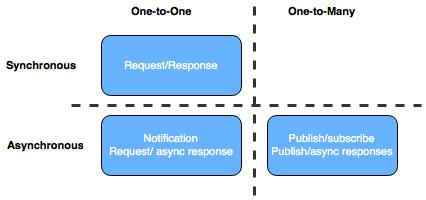
\includegraphics[width=0.8\textwidth]{figures/challenges_one_interaction_styles}
\caption{Inteaction Styles among microservices [\cite{Richardson:2015ab}]}
\label{fig:challanges_of_microservices_architecture/integration/inter_service_communication/interaction_styles_among_microservices}
\end{center}
\end{figure}
\\
\\
\textbf{One to One interactions}
\\
\begin{enumerate}
\item \textbf{Request/Response}: It is synchronous interaction where client sends request and expects for response from server.
\item \textbf{Notification}: It is asynchronous one way interaction where cliend sends request but no reply is sent from server.
\item \textbf{Request/async Response}: It is asynchronous interaction where client requests server but does not block waiting for response. The server send response asynchronously.
\end{enumerate}
\\
\\
\textbf{One to Many interactions}
\\
\begin{enumerate}
\item \textbf{Publish/subscribe}: A service publishes notification which is consumed by other interested services.
\item \textbf{Publish/async responses}: A service publishes request which is consumed by interested services. The services then send asynchronous responses.
\end{enumerate}
\\
\\


\subsubsection{Synchronous and Asynchronous}\label{section:challanges_of_microservices_architecture/integration/synchronous_and_asynchronous}
Each of the interactions listed in section \ref{section:challanges_of_microservices_architecture/integration/inter_service_communication} has its own place in an application. An application can contained a mixture of these interactions. However, a clear idea about the requirement as well as drawbacks associated with the interaction is necessary.\cite{Newman:2015aa}\cite{Richardson:2014aa}\cite{Morris:2015aa}\\
\textbf{Synchronous Interaction}
\\
It is simple to understand to flow and natural easy way of implenting an interaction. However, as the interactions get higher, it increases the overal blocking period of client and thus increasing latency. The synchronous nature of interaction increases temporal coupling between services which demands both to be active at the same time. Since, the synchronous client needs to know the address and port of server to communicate, it also induces location coupling. With the cloud deployment and auto-scaling, this is not simple. Finally, to mitigate the location coupling, service discovery mechanishm is recommended to be used.
\\
  
\textbf{Asynchronous Interaction}
\\
The asynchronous interaction decouples services. It also improves latency as the client is not blocked waiting for the response. However, there is one additional component which is message broker to be managed. Additionally, the conceptual understanding of the flow is not natural, so it is not easy to reason about.

\\
\subsubsection{Example}\label{section:challanges_of_microservices_architecture/integration/example}
The figure shows various interactions during creation of order. At first, the client, 'checkout service' in this case sends Restful Post order request to 'Order service'. Next, the 'order service' publishes 'Order Created' event and then sends response to the client. The 'OrderDetails service', which is subscribed to the event 'Order Created' reponds by first fetching necessary prodcut details from 'Product service' using Restful Get request. Finally, the 'OrderDetails service' sends request to 'Email service' for sending email to customer regarding order details but does not wait for response. The 'Email service' sends response to 'OrderDetails service' when email is sent successfully.
\begin{figure}[H]
\begin{center}
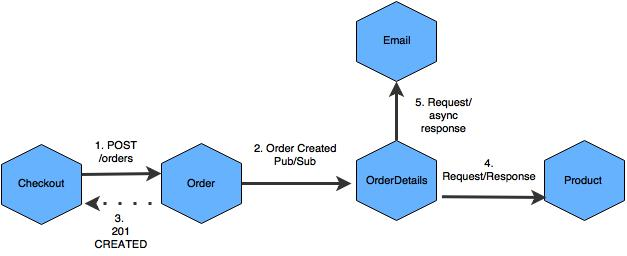
\includegraphics[width=0.8\textwidth]{figures/challanges_two_interaction_example}
\caption{Inteaction during Order creation}
\label{fig:challanges_of_microservices_architecture/integration/inter_service_communication/interaction_during_order_creation}
\end{center}
\end{figure}
\\
\subsection{Breaking Change}\label{section:challanges_of_microservices_architecture/integration/breaking_change}
\\
Although microservices are autonomous components, they still need to communicate. Also, it is obvious that they undergo changes frequently. However, some changes can be backward incompatible and break their consumers. The breaking changes are inevitable but however the impact of the breaking changes can be somehow reduced by applying various techniques. \cite{Newman:2015aa}

\begin{enumerate}
\item Avoid as much as possible \\ A good approach to reduce impact of incompatible changes to the consumers is to defer it as long as it is possible. One way is by choosing the correct integration technology such that loose coupling is maintained. For example, using \acrshort{REST} as an integration technology is better approach than using shared database because it encaptulates the underlying implementation and consumers are only tied to the interfaces.\\
Another approach is to apply TolerantReader pattern while accessing provider's \acrshort{API}. \cite{Fowler:2011aa} Consumer can get liberal while reading data from provider. Without blindly accepting everything from server, it can only filter the required data without carrying about the payload datastructure and order. So, if the reader is tolerant, the consumer service can still work if the provider adds new fields or change the structure of the response.
\item Catch breaking changes early \\ It is also crucial to identify breaking change, if it happens, as soon as  possible. It can be achieved by using consumer-driven contracts. Consumers will write the contract to define the expectations from the producer's \acrshort{API} in the form of various integration tests. These integration tests can become a part of build process of the producer so the breaking change can be detected in the build process before the \acrshort{API} is accessed by the real consumers.
\item Use Semantic Versioning \\ Semantic Versioning is a way to identify the state of current artifact using compact information. It has the form MAJOR.MINOR.PATCH. MAJOR number is increased when backward incompatible changes are made. Similarly, MINOR number is increased when backward compatible functionalities are added. Finally, PATCH number represents that bug fixes are made which are backward compatible.\\
With semantic versioning, the consumers can clearly know if the provider's current update will break their \arshort{API} or not. For example, if consumer is using 1.1.3 version of provider's \arshort{API} and the new updated version is 2.1.3, then the consumer should expect some breaking changes and react accordingly.
\item Coexist Different Endpoints \\ Whenever a breaking change on a service is deployed, it should be carefully considered not to fail all the consumers immediately. One way is to support old version of end points as well as new ones. This will give some time for consumers to react on their side. Once all the consumers are upgraded to use new version of the provider, the old version end point can be removed. However, using this approach means that additional tests to verify both versions.
\item Coexist concurrent service versions \\ Another approach is to support both version of service at once. The requests from old consumers need to be routed to old versioned service and requests from new consumers to the new versioned service. It is mostly used when the cost of updated old consumer is high. However, this also means that two different versions have to be maintained and operated smoothly.
\end{enumerate}
\\
\subsection{Handling Failures}\label{section:challanges_of_microservices_architecture/integration/handling_failures}
With a large number of microservices where communication is happening along not so reliable network, failures are inevitable. At the same time, it becomes challenging as well as highly necessary to handle the failures. Many strategies can be employed for the purpose. \cite{Newman:2015aa}\cite{Richardson:2015ab}\cite{Nygard:2007aa}
\begin{enumerate}
\item Timeouts \\ A service can get blocked indefinitely waiting for response from provider. To prevent this, a threshold value can be set for waiting. However, care should be taken not to choose very low or high value for waiting. 
\item Circuit Breaker \\ If request to a service keep failing, there is less sense to keep sending request to the same server. It can be a better approach to track the request failures and stop sending further request to the service assuming that there is problem with the connection. By failing fast in such a way will not only save the waiting time for the client but also reduces unnecessary network load. Circuit Breaker pattern helps to accomplish the same. A circuit breaker has three states as shown in the figure. In normal cases when the connection to the provider is working fine, it is in 'closed' state and all the connections to the provider goes through it. Once the connection starts failing and meets the threshold (can be number of failures or frequency of failures), the circuit breaker switch to 'open' state. At this state, any more connections fail straight away. After certain time interval, the state changes to 'half open' to check the state of provider again. Any connection request at this point passes through. If the connection is succesful, the state switches back to 'closed' state, else to 'open' state.\cite{Fowler:2014ac} \cite{Newman:2015aa} \cite{Nygard:2007aa}
\begin{figure}[H]
\begin{center}
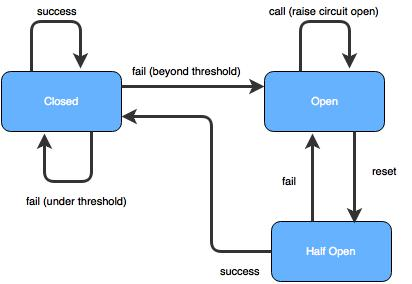
\includegraphics[width=0.8\textwidth]{figures/challanges_three_circuit_breaker}
\caption{States of a circuit breaker [\cite{Fowler:2014ac}]}
\label{fig:challanges_of_microservices_architecture/integration/inter_service_communication/states_of_circuit_breaker}
\end{center}
\end{figure}
\\
\item Bulk Head \\ Bulk Head is the approach of segregating various resources as per requirement and assigning them to respective purposes. Maintaining such threshold in available resources will save any resource from being constrained whenever there is problem in any section. One example of such bulkhead is the assignment of separate connection pool for each downstream resources. In this way, if problem in the request from one connection pool will not affect another connection pool. \cite{Newman:2015aa} \cite{Nygard:2007aa}
\item Provide fallbacks \\ Various fallback logic can be applied along with timeout or circuit breaker to provide alternative mechanism to respond. For example, cached data or default value can be returned. 
\end{enumerate}



















